\documentclass[11pt,a4paper]{article}
\usepackage[utf8]{inputenc}
\usepackage[T1]{fontenc}
\usepackage{lmodern}
\usepackage[portuguese]{babel}
\usepackage[a4paper,margin=2.4cm]{geometry}
\usepackage{xcolor}
\usepackage{graphicx}
\usepackage{titlesec}
\usepackage{enumitem}
\usepackage{listings}
\usepackage{tcolorbox}
\usepackage{booktabs}
\usepackage{amsmath}
\usepackage{amssymb}
\usepackage{fancyhdr}
\usepackage{hyperref}
\tcbuselibrary{skins,breakable,listings}

\definecolor{BgCream}{HTML}{FAF8F5}
\definecolor{TextEspresso}{HTML}{4A4238}
\definecolor{NudeTaupe}{HTML}{BFAFA6}
\definecolor{SoftBlush}{HTML}{D9C5B2}
\definecolor{SageMuted}{HTML}{7E8F7C}
\definecolor{ClayWarn}{HTML}{B5795C}

\hypersetup{colorlinks=true, linkcolor=TextEspresso, urlcolor=TextEspresso}

\titleformat{\section}{\color{TextEspresso}\Large\bfseries}{\thesection}{0.6em}{}[{\color{NudeTaupe}\titlerule[0.8pt]}]
\titleformat{\subsection}{\color{TextEspresso}\large\bfseries}{\thesubsection}{0.6em}{}
\titlespacing*{\section}{0pt}{1.4\baselineskip}{0.7\baselineskip}
\titlespacing*{\subsection}{0pt}{1.1\baselineskip}{0.5\baselineskip}

\lstset{
  basicstyle=\ttfamily\small,
  breaklines=true,
  columns=fullflexible,
  showstringspaces=false,
  frame=none,
  aboveskip=0pt, belowskip=0pt
}

\pagestyle{fancy}
\fancyhf{}
\renewcommand{\headrulewidth}{0pt}
\fancyfoot[C]{\color{NudeTaupe}\small\thepage}

% ---- Caixa: comandos a executar ----
\newtcblisting{terminal}{
  listing only, breakable,
  colback=BgCream, colframe=NudeTaupe,
  boxrule=0.5pt, arc=2pt, left=6pt, right=6pt, top=5pt, bottom=5pt,
  listing options={basicstyle=\ttfamily\small, breaklines=true, columns=fullflexible}
}

% ---- Caixa: saida esperada ----
\newtcblisting{saida}{
  listing only, breakable,
  colback=white, colframe=SoftBlush,
  boxrule=0.5pt, arc=2pt, left=6pt, right=6pt, top=5pt, bottom=5pt,
  title={\small\bfseries\color{TextEspresso}Saída esperada},
  coltitle=TextEspresso, colbacktitle=SoftBlush!45,
  fonttitle=\small\bfseries,
  listing options={basicstyle=\ttfamily\footnotesize, breaklines=true, columns=fullflexible}
}

% ---- Caixa: ponto de verificacao ----
\newtcolorbox{verificar}{
  breakable, colback=SageMuted!8, colframe=SageMuted,
  boxrule=0.6pt, arc=2pt, left=7pt, right=7pt, top=6pt, bottom=6pt,
  title={\small\bfseries Confirme antes de avançar},
  coltitle=white, colbacktitle=SageMuted, fonttitle=\small\bfseries
}

% ---- Caixa: aviso ----
\newtcolorbox{atencao}{
  breakable, colback=ClayWarn!8, colframe=ClayWarn,
  boxrule=0.6pt, arc=2pt, left=7pt, right=7pt, top=6pt, bottom=6pt,
  title={\small\bfseries Atenção},
  coltitle=white, colbacktitle=ClayWarn, fonttitle=\small\bfseries
}

% ---- Caixa: nota/contexto ----
\newtcolorbox{nota}{
  breakable, colback=NudeTaupe!10, colframe=NudeTaupe,
  boxrule=0.5pt, arc=2pt, left=7pt, right=7pt, top=6pt, bottom=6pt
}

% ---- Cabecalho do manual ----
\newcommand{\manualtitle}[3]{%
  \thispagestyle{empty}
  \begin{center}
  {\color{NudeTaupe}\rule{\textwidth}{0.5pt}}\\[0.5cm]
  {\LARGE\bfseries\color{TextEspresso} Manual Técnico #1}\\[0.35cm]
  {\large\color{TextEspresso} #2}\\[0.3cm]
  {\normalsize\color{NudeTaupe} Infraestruturas de Computação na Nuvem \quad|\quad #3}\\[0.4cm]
  {\color{NudeTaupe}\rule{\textwidth}{0.5pt}}
  \end{center}
  \vspace{0.4cm}
}

% ---- Entrada de troubleshooting ----
\newcommand{\problema}[1]{\vspace{0.35cm}\noindent{\bfseries\color{TextEspresso}#1}\par\nopagebreak\vspace{0.1cm}}

\setlist[itemize]{itemsep=0.22cm, topsep=0.2cm}
\setlist[enumerate]{itemsep=0.22cm, topsep=0.2cm}

\begin{document}
\manualtitle{10}{Armazenamento Local com LVM e RAID}{Aula 10}

\section*{Como usar este manual}

Vai construir, dentro da sua VM, uma pilha de armazenamento completa: discos $\rightarrow$ RAID $\rightarrow$ LVM $\rightarrow$ sistema de ficheiros. E depois vai partir um disco de propósito para ver o RAID recuperar.

\begin{atencao}
\textbf{O aviso mais importante do semestre.} Os comandos desta aula escrevem diretamente em discos. Aplicar \texttt{mdadm} ou \texttt{pvcreate} ao disco de sistema \textbf{destrói a sua VM}. Confirme \emph{sempre} com \texttt{lsblk} qual é qual antes de executar.
\end{atencao}

\section*{Antes de começar}

\begin{itemize}
  \item[$\square$] VM \texttt{icn-lab} ligada
  \item[$\square$] Acesso à interface web do Proxmox para anexar discos
  \item[$\square$] Privilégios de \texttt{sudo} na VM
\end{itemize}

\section{O armazenamento do Proxmox}

\subsection{Ver os storages configurados}

Na interface web: \textbf{Datacenter} $\rightarrow$ \textbf{Storage}. Registe cada storage e o seu tipo.

Se tiver shell no node:
\begin{terminal}
$ pvesm status
\end{terminal}

\begin{saida}
Name             Type     Status     Total     Used  Available    %
local             dir     active   98.5GiB  21.3GiB    77.2GiB  21.62%
local-lvm     lvmthin     active  794.3GiB 402.1GiB   392.2GiB  50.62%
\end{saida}

\begin{nota}
Se vir \texttt{lvmthin}, o servidor usa \textbf{LVM com thin provisioning} para os discos das VMs -- exatamente o mecanismo que vai construir hoje, uma camada acima.
\end{nota}

\subsection{Onde está o disco da sua VM}

\begin{terminal}
$ qm config <vmid> | grep -E "scsi|virtio|sata"
\end{terminal}

\begin{saida}
scsi0: local-lvm:vm-101-disk-0,size=20G
\end{saida}

\subsection{Anexar quatro discos}

Na interface web: selecione a VM $\rightarrow$ \textbf{Hardware} $\rightarrow$ \textbf{Add} $\rightarrow$ \textbf{Hard Disk}. Crie \textbf{quatro discos de 1 GB}, um de cada vez.

Equivalente por CLI no node:
\begin{terminal}
$ qm set <vmid> --scsi1 <storage>:1
$ qm set <vmid> --scsi2 <storage>:1
$ qm set <vmid> --scsi3 <storage>:1
$ qm set <vmid> --scsi4 <storage>:1
\end{terminal}

\section{Identificar os discos}

\begin{terminal}
$ sudo apt update && sudo apt install -y mdadm lvm2
$ lsblk
\end{terminal}

\begin{saida}
NAME   MAJ:MIN RM  SIZE RO TYPE MOUNTPOINTS
sda      8:0    0   20G  0 disk
|-sda1   8:1    0    1M  0 part
`-sda2   8:2    0   20G  0 part /
sdb      8:16   0    1G  0 disk
sdc      8:32   0    1G  0 disk
sdd      8:48   0    1G  0 disk
sde      8:64   0    1G  0 disk
\end{saida}

\begin{verificar}
Identifique com clareza:
\begin{itemize}
  \item \textbf{Disco de sistema}: o de 20G, com partições e \texttt{MOUNTPOINTS} preenchido (\texttt{/}). \textbf{Nunca lhe toque.}
  \item \textbf{Discos novos}: os de 1G, sem partições e sem pontos de montagem. São estes os alvos.
\end{itemize}
Escreva os nomes dos quatro discos novos antes de continuar: \underline{\hspace{5cm}}
\end{verificar}

\section{Criar o array RAID 5}

\begin{center}
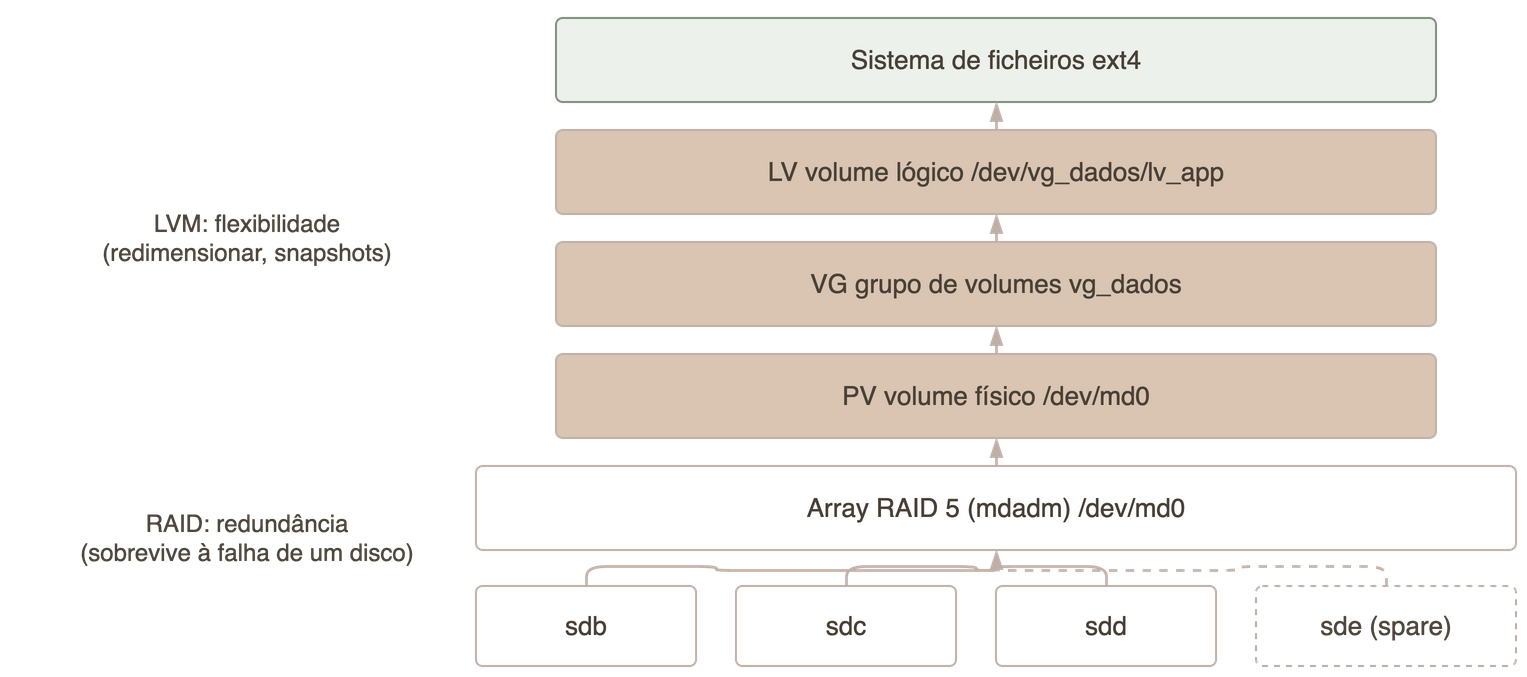
\includegraphics[width=\linewidth]{../Diagramas/a10-pilha-armazenamento.png}\\[0.15cm]
{\small\color{NudeTaupe} As camadas que vai construir, de baixo para cima.}
\end{center}


\begin{terminal}
$ sudo mdadm --create /dev/md0 --level=5 --raid-devices=3 \
    /dev/sdb /dev/sdc /dev/sdd --spare-devices=1 /dev/sde
\end{terminal}

Responda \texttt{y} à confirmação.

\begin{nota}
Três discos em RAID 5 mais um de reserva (\emph{hot spare}). A capacidade útil será a de dois discos: um é ocupado pela paridade distribuída.
\end{nota}

\subsection{Acompanhar a sincronização}

\begin{terminal}
$ cat /proc/mdstat
\end{terminal}

\begin{saida}
Personalities : [raid6] [raid5] [raid4]
md0 : active raid5 sde[3](S) sdd[2] sdc[1] sdb[0]
      2093056 blocks super 1.2 level 5, 512k chunk, algorithm 2 [3/3] [UUU]

unused devices: <none>
\end{saida}

\begin{nota}
Como ler esta saída: \texttt{[3/3]} significa 3 discos esperados, 3 presentes. \texttt{[UUU]} são os estados -- \texttt{U} de \emph{up}; um \texttt{\_} indica um disco em falta. O \texttt{(S)} ao lado do \texttt{sde} identifica o \emph{spare}. Os números entre parênteses retos são os \emph{slots} que cada disco ocupa no array.

Se a criação tiver acabado de decorrer, poderá ainda ver uma linha de \texttt{resync} em progresso -- é normal e não impede a utilização do array.
\end{nota}

\subsection{Guardar a configuração}

\begin{terminal}
$ sudo mdadm --detail --scan | sudo tee -a /etc/mdadm/mdadm.conf
$ sudo update-initramfs -u
\end{terminal}

\section{Construir a pilha LVM}

Ordem: \textbf{PV} (volume físico) $\rightarrow$ \textbf{VG} (grupo) $\rightarrow$ \textbf{LV} (volume lógico).

\subsection{Volume físico}

\begin{terminal}
$ sudo pvcreate /dev/md0
$ sudo pvdisplay
\end{terminal}

\subsection{Grupo de volumes}

\begin{terminal}
$ sudo vgcreate vg_dados /dev/md0
$ sudo vgdisplay vg_dados | grep -E "VG Name|VG Size|Free"
\end{terminal}

\subsection{Volume lógico}

\begin{terminal}
$ sudo lvcreate -l 80%VG -n lv_app vg_dados
$ sudo lvdisplay /dev/vg_dados/lv_app
\end{terminal}

\begin{atencao}
Usamos \textbf{80\%} e não 100\% de propósito: o snapshot que vamos criar precisa de espaço livre no grupo de volumes. Se ocupar tudo agora, o snapshot falha.
\end{atencao}

\subsection{Formatar e montar}

\begin{terminal}
$ sudo mkfs.ext4 /dev/vg_dados/lv_app
$ sudo mkdir -p /mnt/dados
$ sudo mount /dev/vg_dados/lv_app /mnt/dados
$ df -h /mnt/dados
\end{terminal}

\begin{verificar}
O \texttt{df -h} mostra o volume montado em \texttt{/mnt/dados}. Percorreu toda a pilha: quatro discos virtuais transformaram-se num sistema de ficheiros utilizável.
\end{verificar}

\section{Snapshots}

\subsection{Criar dados}

\begin{terminal}
$ echo "versao inicial" | sudo tee /mnt/dados/ficheiro.txt
$ cat /mnt/dados/ficheiro.txt
\end{terminal}

\subsection{Criar o snapshot}

\begin{terminal}
$ sudo lvcreate -L 200M -s -n lv_app_snap /dev/vg_dados/lv_app
$ sudo lvs
\end{terminal}

\begin{saida}
  LV          VG       Attr       LSize   Pool Origin Data%
  lv_app      vg_dados owi-aos---   1.60g
  lv_app_snap vg_dados swi-a-s--- 200.00m      lv_app  0.01
\end{saida}

\begin{nota}
Repare na coluna \texttt{Data\%} do snapshot: praticamente zero. O snapshot ainda não copiou nada. Só copiará os blocos que forem alterados no original -- é o \emph{copy-on-write}.
\end{nota}

\subsection{Alterar o original}

\begin{terminal}
$ echo "versao alterada" | sudo tee /mnt/dados/ficheiro.txt
$ sudo lvs vg_dados/lv_app_snap
\end{terminal}

O \texttt{Data\%} subiu: o bloco alterado foi copiado para o snapshot.

\subsection{Montar o snapshot e comparar}

\begin{terminal}
$ sudo mkdir -p /mnt/snapshot
$ sudo mount -o ro /dev/vg_dados/lv_app_snap /mnt/snapshot
$ echo "--- ORIGINAL ---"; cat /mnt/dados/ficheiro.txt
$ echo "--- SNAPSHOT ---"; cat /mnt/snapshot/ficheiro.txt
\end{terminal}

\begin{saida}
--- ORIGINAL ---
versao alterada
--- SNAPSHOT ---
versao inicial
\end{saida}

\begin{verificar}
O snapshot preservou o estado anterior. É assim que se obtêm backups consistentes de um volume em uso, sem parar a aplicação.
\end{verificar}

\section{Simular a falha de um disco}

\subsection{Marcar como falhado}

\begin{terminal}
$ sudo mdadm --manage /dev/md0 --fail /dev/sdc
$ cat /proc/mdstat
\end{terminal}

\begin{saida}
md0 : active raid5 sde[4] sdd[2] sdc[1](F) sdb[0]
      2093056 blocks super 1.2 level 5, 512k chunk, algorithm 2 [3/2] [U_U]
      [======>..............]  recovery = 32.5% (340608/1046528) finish=0.0min
\end{saida}

\begin{verificar}
Três coisas aconteceram de imediato:
\begin{itemize}
  \item \texttt{sdc} passou a \texttt{(F)} -- \emph{failed}
  \item O \emph{spare} \texttt{sde} deixou de ter o \texttt{(S)} e passou a ocupar um slot ativo
  \item O array ficou \texttt{[3/2]} e \texttt{[U\_U]} -- \textbf{degradado}
  \item A reconstrução começou \textbf{sozinha}, usando o \emph{hot spare}
\end{itemize}
\end{verificar}

\subsection{Confirmar que os dados continuam acessíveis}

\begin{terminal}
$ cat /mnt/dados/ficheiro.txt
$ echo "escrito durante a reconstrucao" | sudo tee -a /mnt/dados/ficheiro.txt
\end{terminal}

\begin{nota}
O serviço nunca parou. É exatamente para isto que serve o RAID: sobreviver à falha de um disco sem interrupção. Com discos de 1 GB a reconstrução é quase instantânea; em produção, com discos de vários terabytes, demoraria horas ou dias -- e durante todo esse tempo o array estaria degradado e vulnerável a uma segunda falha.
\end{nota}

\subsection{Substituir o disco}

\begin{terminal}
$ sudo mdadm --manage /dev/md0 --remove /dev/sdc
$ sudo mdadm --manage /dev/md0 --add /dev/sdc
$ cat /proc/mdstat
$ sudo mdadm --detail /dev/md0 | tail -8
\end{terminal}

O \texttt{sdc} passou a ser o novo \emph{spare}.

\section{Problemas frequentes}

\problema{Os discos novos não aparecem no \texttt{lsblk}}
Reinicie a VM (\texttt{sudo reboot}). Alguns controladores só detetam discos novos no arranque. Confirme também no Proxmox, separador \emph{Hardware}, que os discos foram mesmo criados.

\problema{\texttt{mdadm: /dev/sdb appears to be part of a raid array}}
Restos de uma tentativa anterior. Limpe as assinaturas (\textbf{confirmando que é o disco certo}):
\begin{terminal}
$ sudo mdadm --zero-superblock /dev/sdb
\end{terminal}

\problema{\texttt{mdadm: cannot open /dev/sdb: Device or resource busy}}
O disco está em uso. Pare o array primeiro:
\begin{terminal}
$ sudo umount /mnt/dados
$ sudo mdadm --stop /dev/md0
\end{terminal}

\problema{\texttt{Insufficient free space} ao criar o snapshot}
O volume lógico ocupou todo o grupo. Confirme o espaço livre:
\begin{terminal}
$ sudo vgs
\end{terminal}
Se \texttt{VFree} for zero, reduza o LV ou recrie-o com 80\%.

\problema{O snapshot fica cheio e é invalidado}
Um snapshot só tem o espaço que lhe foi atribuído. Se o original mudar mais do que isso, o snapshot torna-se inutilizável (\texttt{Attr} com \texttt{I}). Crie-o com mais espaço, ou não altere tanto o original.

\problema{\texttt{mount: unknown filesystem type}}
Esqueceu-se do \texttt{mkfs.ext4}. Um volume lógico acabado de criar não tem sistema de ficheiros.

\problema{O array desaparece depois de reiniciar}
Faltou guardar a configuração. Repita:
\begin{terminal}
$ sudo mdadm --detail --scan | sudo tee -a /etc/mdadm/mdadm.conf
$ sudo update-initramfs -u
\end{terminal}

\problema{Montei o snapshot sem \texttt{-o ro} e agora dá erro}
Um snapshot deve ser montado só de leitura. Desmonte e volte a montar com \texttt{-o ro}.

\section{Referência rápida}

\begin{center}
\begin{tabular}{@{}ll@{}}
\toprule
\textbf{Comando} & \textbf{Para que serve} \\
\midrule
\texttt{lsblk} & Ver discos e partições \\
\texttt{cat /proc/mdstat} & Estado dos arrays RAID \\
\texttt{mdadm -{}-detail /dev/md0} & Detalhe completo do array \\
\texttt{mdadm -{}-manage /dev/md0 -{}-fail X} & Marcar disco como falhado \\
\texttt{mdadm -{}-manage /dev/md0 -{}-remove X} & Remover disco do array \\
\texttt{mdadm -{}-manage /dev/md0 -{}-add X} & Acrescentar disco \\
\midrule
\texttt{pvcreate} / \texttt{pvs} & Criar / listar volumes físicos \\
\texttt{vgcreate} / \texttt{vgs} & Criar / listar grupos de volumes \\
\texttt{lvcreate} / \texttt{lvs} & Criar / listar volumes lógicos \\
\texttt{lvcreate -L T -s -n nome LV} & Criar snapshot \\
\texttt{mkfs.ext4 <dispositivo>} & Formatar \\
\texttt{mount} / \texttt{umount} & Montar / desmontar \\
\texttt{df -h} & Espaço nos sistemas de ficheiros montados \\
\bottomrule
\end{tabular}
\end{center}

\section{Checklist final}

\begin{itemize}
  \item[$\square$] Registei os storages do Proxmox e onde reside o disco da minha VM
  \item[$\square$] Anexei quatro discos e identifiquei-os com segurança no \texttt{lsblk}
  \item[$\square$] Criei o array RAID 5 com hot spare e sei ler o \texttt{/proc/mdstat}
  \item[$\square$] Construí PV, VG e LV, e deixei 20\% livres no VG
  \item[$\square$] Formatei e montei o volume em \texttt{/mnt/dados}
  \item[$\square$] Criei o snapshot, alterei o original e comparei os dois conteúdos
  \item[$\square$] \textbf{Marquei um disco como falhado e vi o hot spare entrar sozinho}
  \item[$\square$] Confirmei que os dados continuaram acessíveis durante a reconstrução
  \item[$\square$] Substituí o disco falhado
  \item[$\square$] Guardei as saídas de \texttt{mdadm --detail}, \texttt{vgdisplay} e \texttt{lvdisplay}
\end{itemize}

\end{document}
